\documentclass{./Templates/llncs/llncs}
\usepackage{./Templates/llncs/llncsdoc}

\usepackage{graphicx}
\usepackage{subfig}
\usepackage{url}
\usepackage{algorithm}
\usepackage{algorithmic}
\usepackage{listings}
\usepackage{amsmath}
\usepackage{amsthm}
\usepackage{verbatim}
%Percom: for other experimental results
\graphicspath{{./figures/}{./simulation/}{../figures/psware/}{../figures/shm/}{../simulation/psware/}}
\newcommand{\HRule}{\rule{\linewidth}{0.5mm}}
%\newcommand{\figurecurrentwidth}{\includegraphics[width=\textwidth]}
%\newcommand{\figurehalfwidth}{\includegraphics[width=.5\textwidth]}
\newcommand{\figurecurrentwidth}{\includegraphics[width=\textwidth]}
\newcommand{\figurehalfwidth}{\includegraphics[width=.5\textwidth]}
\lstset{float, numbers=left, frame=lines, belowcaptionskip=3mm, xleftmargin=7mm, framexleftmargin=7mm, escapeinside={(*}{*)}, tabsize=3, breaklines=true}
\renewcommand{\algorithmicrequire}{\textbf{Input:}}
\renewcommand{\algorithmicensure}{\textbf{Output:}} 
\pdfminorversion=9

\hyphenation{op-tical net-works semi-conduc-tor}

\begin{document}

\title{PSWare: A Flexible Middleware Framework for Composite Event in Wireless Sensor Network}
\author{
{Scribus Primus}\\
\affaddr{Primus Address}\\
\email{primus@somewhere.com} \and
{Scribus Secundus}\\
\affaddr{Secundus Address}\\
\email{secondus@elsewhere.com}
}
\conferenceinfo{SenSys'11,} {November 1--4, 2011, Seattle, WA, USA.}
\CopyrightYear{2011}
\crdata{XXX-X-XXXXX-XXX-X}
\maketitle
\begin{abstract}
Event detection is an important topic in many WSN applications. Although there are several works on providing event-based services in WSN, most of them can only deal with primitive event types but cannot handle composite events very well. In general, a type-based event system may have primitive or composite event types. All event types are defined by specifying their attributes and filters. Then, individual events are detected and delivered according to such type information. Composite event types may be defined by combining multiple event types with operators. Due to the resource constraints in WSN, composite events are much more difficult to manage than primitive events. In this work, we introduce PSWare, a type-based publish / subscribe middleware for WSN that supports composite events. We describe our design for PSWare. PSWare has a flexible architecture where different composite event detection algorithms may be easily integrated.

On top of PSWare, we present TED (Type-based Event Detection), a novel distributed composite event detection algorithm. The essential idea of TED is event fusion, where some sensor nodes are selected as fusion points and component events are fused for the detection of a high level event. Event fusion with minimum energy cost is an NP-complete problem. Therefore, TED uses a number of heuristics with bounded performance.  

To further increase the performance of event detection, we design a clustering algorithm for PSWare for structural health monitoring applications (SHM). We formulate the problem and found it to be NP-complete so we propose heuristic centralized and distributed algorithms. In addition to SHM, We use PSWare to develop other real world WSN applications including intelligent transportation system (ITS) and in-door monitoring.

We evaluate our system from different aspects. We first evaluate TED, the most essential algorithm in our system. We analyze its performance and then carry out extensive simulations. Both analytical and simulation results show TED can save energy in event-based applications where primitive events occur in a higher frequency than composite events. Then we combine TED with PSWare and carried out some real world experiments. The results show that PSWare can offer reasonably simple API for the application developers to use while TED and our clustering algorithm can improve the underlying event detection performance. Compared with opportunistic approaches to event detection in these real applications, PSWare can reduce 40 - 50 \% of the energy cost.
\end{abstract}
\chapter{Introduction}
\section{Overview}
\label{sec:introduction}
Development in wireless communication and electronics has made it possible to create low-cost, low-power wireless sensor nodes. Each sensor node usually contains a wireless transceiver, a micro processing unit and a number of sensors. The sensor nodes can collect data and do some simple processing locally, and can communicate with each other to form an ad hoc wireless sensor network (WSN) \cite{aky:survey}. A WSN is usually self-organized and self-maintained without any human intervention. Wireless sensor networks have been used in various application areas such as smart building \cite{lynch:shm}, wild environment monitoring \cite{wsnhabitat}, intelligent transportation systems \cite{klein:its}, battle surveillance \cite{wsntracking} and healthcare \cite{lo:ban}. 

While WSN has a wide range of applications, programming sensor networks is a challenging because different from programming in the traditional environment. WSN imposes a lot of constraints such as limited computational power, less memory and unreliable communication. Application developers need to not only understand the requirements for the specific application domain but also take into consideration of the characteristics of WSN. In this research work, we propose PSWare, a publish/subscribe (pub/sub) middleware for WSN which eases the development of WSN applications. Our middleware uses a pub/sub programming paradigm for the application programmer to subscribe application specific events. It provides an easy-to-use Event Definition Language (EDL) to allow the application developers to define composite events while uses a flexible architecture so that different domain-specific event processing algorithms can be easily integrated into the middleware.

\subsection{Motivation}
Despite the large variety of WSN applications, many of them are essentially event-based. In applications such as intelligent transportation systems \cite{klein:its}, smart buildings \cite{lynch:shm} and healthcare \cite{lo:ban}, the events sensor nodes detect events which reflect the environmental changes and the systems respond to these events accordingly. Events may be primitive or composite. Primitive events (e.g. when the temperature exceeds certain threshold) can be detected by a single sensor node without having to cooperate with others. On the other hand, \emph{composite events} consist of multiple primitive events. They reflect a serial of environmental changes with spatial and temporal relations among them and must be detected collaboratively by different sensor nodes.

Because of the common requirements and challenges for composite event subscription and detection, it is more desirable to have a generic middleware layer to handle composite events instead of reinventing the wheel and implementing application-specific event processing mechanisms. In addition, the middleware should be flexible enough so that different event processing algorithms for different application domains can be easily integrated. In summary, the middleware should achieve the following design goals:
\begin{enumerate}
\item \emph{Event abstraction}: since composite events are collaboratively processed by different sensor nodes in the network, they introduce extra complexity because of the resource constraints and unreliable communication. A middleware framework providing high level event abstraction is needed to ease the application development.
\item \emph{Re-usability and flexibility}: different applications may share certain common modules during event processing. They may also have other different modules. A middleware framework can help so that common modules may be used and different modules may be replaced without affecting others.
\end{enumerate}

\subsection{Issues}
In this research, we address the essential issues of designing and developing PSWare. On the highest level, an event description language is provided to allow users to describe composite event relationships. On the lowest level, a runtime environment is necessary on each sensor nodes so that they could understand and execute the event processing algorithms translated from the high-level EDL. More specifically, we need to address the following research/engineering issues to make our middleware work.

\begin{itemize}
\item	\emph{Event definition language}: we need to provide an event description language which is powerful yet easy to use.
\item	\emph{Event definition language compiler}: a compiler is essential to translate the programs written in our high-level language into a low-level language understandable by the sensor nodes. The compiler must be smart enough to extract the semantic meanings from the program and do some optimization.
\item	\emph{Runtime environment support}: the middleware running on each sensor node should provide a runtime environment to execute the compiled programs.
\item	\emph{Subscription propagation}: after the program written in EDL is compiled, the subscription should be intelligently disseminated into the network. If the subscription is too big, it may need to be divided into small ones. Furthermore, only related sensor nodes need to be updated.
\item	\emph{Event detection}: we need to design efficient protocol for the sensor nodes to cooperate with each other to detect composite events.
\item	\emph{Event delivery}: after the subscribed the events have been detected, we need energy-efficient routing protocols so that the detected events will be delivered at the minimum cost.
\end{itemize}
\section{Related Works}
\label{sec:relatedworks}
Existing works on pub/sub systems for WSN primarily consider the detection of primitive events where each event is usually treated separately and events don't have relations between each other. \cite{lowlevelnaming} is a pub/sub system built on top of directed diffusion \cite{directeddiffusion}. The sink node will first broadcast interest and the source nodes will deliver the detected events through gradients and reinforced paths. Mires \cite{mires} is a pub/sub middleware for WSN. It makes use of the message-oriented communication paradigm provided by TinyOS \cite{nesc}. First, nodes will advertise their available topics using a multi-hop routing protocol. Then, the sink will broadcast the subscription and finally, nodes will be able to publish the events to the sink. \cite{sp} had an in-depth discussion on the trade-off between reliability and energy consumption. Instead of flooding the subscription to every node in the network, the flood stops after certain number of hops. If the subscription does not reach the publisher, then the event will be forwarded probabilistically. 

More recently, certain works such as \cite{lai:ted, complexevent} have been proposed for composite event definition and detection. The primary focus of \cite{lai:ted} is on a composite event detection algorithm called TED which utilizes event type information for efficient detection. In addition to an event language, \cite{complexevent} also discusses how to reliably detect composite events in a pervasive environment. The focus of this paper is on a flexible middleware framework so that different event detection algorithms may be integrated and evaluated easily.

Apart from the pub/sub paradigm, there have been a lot of efforts on developing other type of programming abstractions for WSN including query-based approaches \cite{cougar, sina, tinydb} VM-based approaches \cite{magnetos, mate, smartmessage} tuple space-base approaches \cite{tinylime} neighbor-based approach \cite{kairos, hood, abstractregion} and mobile agent-based approaches \cite{agilla, sensorware}.

In terms of composite event detection in WSN, there have been very limited works. However, a lot of work has been done on data aggregation for sensor network. Existing data aggregation can be mainly divided into three categories: cluster-based approach \cite{leach, iheed, epas}, chain-based approach \cite{pegasis} and tree-based approach \cite{mfst, dctc, tag, xue:lp, tina}. Cluster-based approach typically considers the problem how to select and rotate cluster heads so that the clusters can be evenly distributed in the network \cite{iheed} and energy consumption will be balanced \cite{leach}. Cluster-based approach can be organized into multiple levels in order to further save the cost. Chain-based approach improves cluster-based approach by letting each sensor node only communicate with its close neighbors \cite{pegasis}. Tree-based approaches have many differnt optimizatin techniques. For example, \cite{xue:lp} formulates the problem as a multi-commodity flow problem and uses linear programming to solve it.  MFST \cite{mfst} constructs a minimum Steiner tree with a cost model that considers the fusion cost. 

We believe the pub/sub paradigm is suitable for many WSN applications because many of these applications are event-based in nature. However, more work needs to be done in order to support efficient composite event detection, especially how to support application-specific event detection mechanisms so that high energy efficiency can be achieved.
\begin{figure}
\centering
\figurecurrentwidth{psware-architecture}
\caption{Event processing in PSWare}
\label{fig:psware-architecture}
\end{figure}

\section{Composite Event Processing in PSWare}
\label{sec:design}
In this section, we discuss how PSWare is designed to support composite event. The overall work flow of event processing in PSWare is shown in Figure \ref{fig:psware-architecture}. To use the middleware, applications developers will first define event types according to the application requirements. The subscription will then be compiled and processed by the EDL compiler and be disseminated into the network. When the events are detected by the sensor nodes, they will be delivered to the application.

\subsection{Event Specification}
\begin{figure}
\centering
\figurecurrentwidth{edlcompiler}
\caption{PSWare-EDL compiler structure}
\label{fig:edlcompiler}
\end{figure}

EDL is used for specifying events in PSWare. For each EDL script, it contains one or more event definition and one subscribing statement. Formally, the BNF of the subscription is defined in Listing \ref{lst:BNFSubscription}.

\begin{lstlisting}[caption=BNF (simplified) of subscription, label=lst:BNFSubscription]
subscription -> event_declarations subscribe_statement
event_declarations -> event_declaration | event_declarations event_declaration
subscribe_statement -> SUBSCRIBE IDENTIFIER SEMICOLON
\end{lstlisting}

The subscribe statement simply uses the keyword 'subscribe' followed the event type name needed by the application. Each event type declaration can have up to three parts: the event body, the where clause and the on clause. The event body defines the attributes of the events. The on clause are used to specify the sub-events used by a composite event. The where clause defines the filter of the corresponding event type. Formally, the BNF of event type is defined in Listing \ref{lst:BNFEvent}

\begin{lstlisting}[caption=BNF (simplified) of event type, label=lst:BNFEvent]
event_declaration -> EVENT IDENTIFIER event_body on_clause_opt where_clause_opt
event_body -> { field_declarations_opt }
on_clause -> ON { subevent_declarations_opt }
where_clause -> WHERE { conditional_expression }
\end{lstlisting}

The on clause and the where clause are both optional in case if the event is primitive or does not have a filter. The on clause looks similar to the field declaration except sub-events instead of fields are declared. This is done for a clear code presentation and easier type checking. The where clause simply consists of conditional expressions so that the filters may be defined by specifying the operators.

\begin{comment}
A simple example of using EDL is shown in Listing \ref{lst:originaledl}. In this example, two events, 'SimpleEvent' and 'CompEvent' are defined. 'SimpleEvent' is a primitive event which occurs when the detected temperature reading is above certain threshold. 'CompEvent' is a composite event that is based on two events of 'SimpleEvent' and their time must satisfy a certain condition in order to indicate the occurrence of 'CompEvent'.
\begin{lstlisting}[caption=A simple EDL program, label=lst:originaledl]
Event SimpleEvent {
	int temp=System.temp;
	int id=System.id;
	int time=System.time;
} where {
	temp > 30
}
Event CompEvent {
} on {
	SimpleEvent e1 and
	SimpleEvent e2
} where {
	e2.time-e1.time=600
}
\end{lstlisting}
\end{comment}

The EDL-based subscription will be processed by our EDL compiler. The output of the compiler has two parts as shown in Figure \ref{fig:edlcompiler}. The first part is the byte codes which will be executed by individual sensors to detect events. The format and the organization of the byte codes are closely related to the event processing framework and customization of PSWare. We will go through these topics in the following sections.

\begin{figure}
\centering
\figurecurrentwidth{edlcompiler-flow}
\caption{EDL compiler flow}
\label{fig:edlcompiler-flow}
\end{figure}

The second part, the event receiving module is the implementation of the event notifier as discussed in Section \ref{sec:model}. As shown in Figure \ref{fig:edlcompiler-flow}, The EDL compiler will execute the following steps in order to generate the byte codes and event receiving module:
\begin{enumerate}
\item Parse the EDL script and generate the corresponding syntax tree and symbol table.
\item Generate the byte codes based on the syntax tree and symbol table.
\item Create the event receiving module based on the symbol table.
\end{enumerate}

\subsection{Runtime Environment for Event Detection}
The byte codes generated by the compiler can be further divided into three parts: event meta data, event filters and event matcher. These components implements the programming interface discussed in Listing \ref{lst:pswareAPI} and \ref{lst:pswareEventMatcher}. Event meta data contains the description of the event types such as event type ID, event size and the individual attributes for each event. Event filters are the constraints defined for each event type. Event matcher schedules the execution for event detection according to the subscription and event relations.

The runtime environment on each sensor node is similar to the VM-based approach \cite{mate} in the sense that the subscriptions are broken down into some basic operations called instructions. Such design choice is for extensibility so that new features can be added more easily by adding new instructions. In addition to the VM-based runtime environment, each sensor node has an event buffer where the detected events can be stored for composite event detection.

\begin{figure}
\centering
\figurecurrentwidth{eventdetectionframework2}
\caption{PSWare runtime environment}
\label{fig:eventdetectionframework2}
\end{figure}
The essential operations for our runtime environment is shown in Figure \ref{fig:eventdetectionframework2}. In this environment, the event matcher will first fetch the events from the event buffer and then evaluate them against the corresponding filters. If the event has been detected, then it will be transmitted over the network. Formally, the procedure of the event matcher can be shown in Procedure \ref{algo:eventmatcher} with some notations defined as:
\begin{itemize}
\item Event types: \(E=\{e_1, e_2 \cdots \}\)
\item For each \(e_n\in E\), its filter is: \(e_n\rightarrow filter\)
\item For each \(e_n\in E\), it has a set of events \(E_n=\{e_n^1, e_n^2 \cdots \}\) stored in the buffer.
\end{itemize}

\begin{algorithm}
\begin{algorithmic}
\REQUIRE \(E\)
	\FORALL {\(e_n\in E\)}
		\FORALL {\(e_n^i\in E_n\)}
			\IF {\(e_n\) is primitive}
				\STATE result = evaluate\_primitive (\(e_n^i\))
				\IF {result == True}
					\STATE eventMatched(\(e_n^i\))
					\IF {\(e_n\) is subscribed}
						\STATE deliver(\(e_n^i\))
					\ELSE
						\STATE forward(\(e_n^i\))
					\ENDIF
				\ENDIF
			\ELSE
				\STATE \(e_{sub} = \emptyset \)
				\FORALL {subevents \(e_m\) for \(e_n\)}
					\STATE \(e_{sub} = e_{sub}\bigcup selectSubevent (e_n, e_m)\)
				\ENDFOR
				\FORALL {subevents \(e_m\) for \(e_{sub}\)}
					\STATE evaluate\_composite(\(e_n^i\), \(e_m\), \(\cdots \))
				\ENDFOR
			\ENDIF
		\ENDFOR
	\ENDFOR
\end{algorithmic}
\caption{Procedure of the event matcher}
\label{algo:eventmatcher}
\end{algorithm}

There are several keys in the procedure. First, when the event matcher picks up the events of type \(e_n\) from the event buffer, it may use application specific mechanisms to pick up the desired events instead of trying all the possible combinations. Second, the 'deliver()' and the 'forward()' function are used to deliver the subscribed events or forward the events so that composite events may be detected. These two functions may also be application dependent to achieve high energy efficiency.

\begin{comment}
Figure \ref{fig:psware-interaction-simple} illustrates how different components in the middleware system interact with each other.

\begin{figure}
\centering
\figurecurrentwidth{psware-interaction-simple}
\caption{PSWare-E components interaction}
\label{fig:psware-interaction-simple}
\end{figure}
\subsection{PSWare Customization}
\end{comment}

Finally, it is necessary to mention the 'SystemEvent'. This module acts as the device driver for PSWare. It defines the sampling rate and a primitive event. All the fields of other events are obtained from 'System'. The module needs to implement three interfaces: StdControl, SystemClock and SystemEvent as shown in Listing \ref{lst:systemEvent}. StdControl is a module for initialization purpose. SystemClock defines the sampling frequency. SystemEvent is used to obtain the pointer to the 'System' event.

\begin{lstlisting}[caption=API of the 'System' event, label=lst:systemEvent]
module SystemEventM {
	provides {
		interface StdControl;
		interface SystemEvent;
		interface SystemClock;
	}
}
interface SystemEvent {
	command EventInstanceInfo * get();
}
\end{lstlisting}

The 'SystemEvent' is there so that needs to be implemented by the middleware developers as the  Once the 'System' event is defined, the application developers can further define their own functions for event delivery and event forwarding. We will show some examples in the next section. 
\section{Evaluation}
\label{sec:experiments}
In this section, we evaluate PSWare. We first introduce the metrics we use for performance evaluation. Then, we present the evaluation results based on the three application cases discussed in the previous section. 

\subsection{Performance Metrics}
The primary of PSWare is help developing WSN-based applications. However, additional overhead may be introduced by its event detection framework. Therefore, we use the following metrics to evaluate PSWare:
\begin{itemize}
\item Memory usage: since the sensor nodes have limited amount of memory, it is important to know the memory overhead introduced by PSWare in order to evaluate its practical use. 
\item Message cost: it is useful to measure the application message cost when using customized event processing mechanism. This way, we can show how PSWare is helpful in deploying real applications. The message cost is obtained by setting up a counter inside the sensor node. The counter will be written into flash so that we can retrieve it after the experiments.
\item Event detection delay: some event processing mechanisms aims at shortening the event detection delay. In this paper, we measure the time between the subscription is disseminated and the event is notified.
\end{itemize}

For each of the application case discussed in the previous section, we implemented an additional opportunistic event detection mechanism where all the events are transmitted to the sink for detection. The transmission is done using the existing routing protocol, CTP, provided by TinyOS. This serves as reference when studying the performance.

\subsection{Results}
In the car park application, the messages indicating the occupancy of the cars must be reliably delivered to the control center. Therefore, we implemented a retransmission mechanism for event delivery. With PSware, the application takes 61k bytes of code and 1.5k bytes of data. Without PSWare, the application takes around 35k bytes for code and 1.3k bytes for data. For the evaluation, we primarily consider only the message costs because the delay isn't that important in such a system. The experimental results for the car park are shown in Figure \ref{fig:carParkResults}. The message cost is highest during rush hour when there are a lot of cars entering and leaving the car park. To further study application under different settings, we used two deployment strategies. The first one is even deployment, where all the parking spaces in a particular area are deployed. In the second strategy, we assume the management is only interested in a subset of the parking spaces so we randomly deployed the sensor nodes in some of the parking spaces. For all the experiments as we can see, the message cost by using application-specific middleware for ITS is the lowest while the opportunistic way is the highest.

\begin{figure}
\centering
\subfloat[With random fusion point deployment]{\label{fig:carParkResult1}\figurehalfwidth{carParkResult1}}
%\qquad
\subfloat[With even fusion point deployment]{\label{fig:carParkResult2}\figurehalfwidth{carParkResult2}}
\caption{Car park experiment results}
\label{fig:carParkResults}
\end{figure}

The next application we evaluate is ITS. One distinct feature of ITS is that we can make use of the special road deployment of the sensor nodes to make event processing easier. As a result, by replacing the default event processing algorithm with a simpler one that processes the event along the road, both code and data sizes are reduced. Without PSWare, the application takes around 25k bytes for code and 1.2k bytes for data. With PSware, it takes around 51k bytes of code and 1.4k bytes of data. The results for ITS are shown in Figure \ref{fig:itsResults}. Different from the car park application, such applications are more delay sensitive. So we also measured the time delay for the event detection. %Similar to the car park application, ITS-specific event detection mechanism can save most energy. Both ITS and TED will introduce certain amount of delay due to the waiting.
 
\begin{figure}
\centering
\subfloat[Message cost]{\label{fig:itsResult1}\figurehalfwidth{itsResult1}}
%\qquad
\subfloat[Delay]{\label{fig:itsResult2}\figurehalfwidth{itsResult2}}
\caption{Experiments on the roads}
\label{fig:itsResults}
\end{figure}

Our final experiments is for the indoor monitoring application. We consider the application scenario where the sensor nodes are deployed in a building so that the temperature can be monitored. With PSware, the application takes 58k bytes of code and 1.5k bytes of data. Without PSWare, the application takes around 34k bytes for code and 1.3k bytes for data. The application As discussed in the previous sections, such an application can probably be useful for certain types of context aware pervasive applications such as indoor temperature monitoring. The experimental results is shown in Figure \ref{fig:itsResults}. 

\begin{figure}
\centering
\subfloat[With random fusion point deployment]{\label{fig:indoorResult1}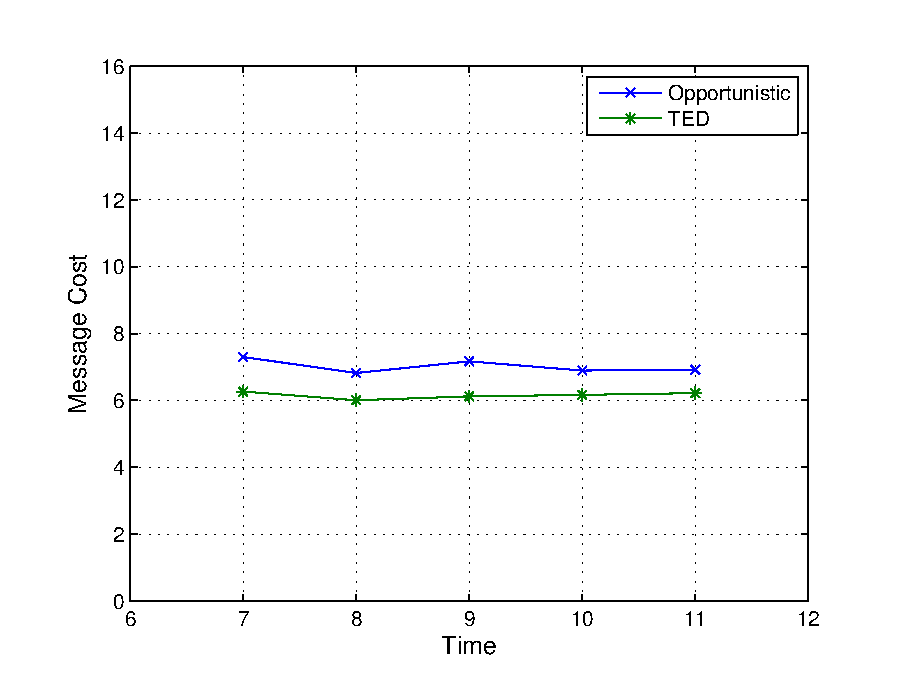
\includegraphics[width=.5\textwidth]{indoorResult1}}
%\qquad
\subfloat[With even fusion point deployment]{\label{fig:indoorResult2}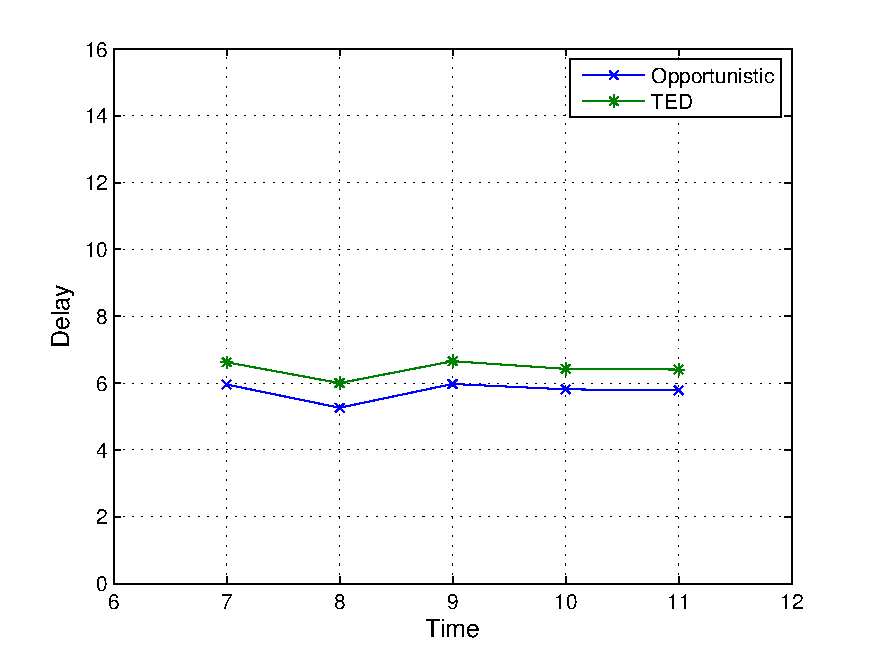
\includegraphics[width=.5\textwidth]{indoorResult2}}
\caption{Experiments for temperature monitoring}
\label{fig:indoorResult}
\end{figure}

\section{Conclusion}
\label{sec:conclusion}
In this paper, we presented PSWare, a flexible middleware framework for composite events processing. PSWare uses a flexible architecture where different event detection mechanisms may easily integrated. We described the design of PSWare and explained how it can be customized for different applications. Then we gave two examples of using PSWare. The first one implements a more general composite event algorithm while the second one uses an application-specific event detection approach. Based on our implementation, we performed experiments and demonstrate the effectiveness of PSWare for prototyping and performance comparison.

\bibliographystyle{./Templates/llncs/splncs03}
\bibliography{../references/wsn-general,../references/wsn-aggregation,../references/wsn-middleware,../references/wsn-pubsub,../references/edl,../references/pubsub,../references/algorithms,../references/event-detection,../references/pervasive,../references/shm}

\end{document}